% Самостоятельная методичка лекции 8. Сборка из корня:
% latexmk 8/finite-maneuvers.tex
\documentclass[a4paper,11pt]{article}
\usepackage{iftex}
\RequirePDFTeX
\usepackage{cmap}
\usepackage[T2A]{fontenc}
\usepackage[utf8]{inputenc}
\usepackage[english,russian]{babel}
\usepackage{PTSerif}
\usepackage{amsmath,amssymb,amsthm,mathtools}
\usepackage[a4paper,left=20mm,right=20mm,top=22mm,bottom=23mm,headheight=14pt]{geometry}
\usepackage{microtype}
\usepackage{graphicx,xcolor,tikz,booktabs,tabularx,array,longtable}
\usetikzlibrary{arrows.meta,calc,positioning}
\usepackage{enumitem,fancyhdr,needspace,float,placeins}
\usepackage[most]{tcolorbox}
\definecolor{accent}{HTML}{187AA5}
\definecolor{muted}{HTML}{5A6166}
\definecolor{figink}{HTML}{25323F}
\definecolor{figtan}{HTML}{087F78}
\definecolor{figorange}{HTML}{B57714}
\definecolor{figpurple}{HTML}{79539C}
\newtcolorbox{explanation}[1]{enhanced,
 colback=accent!3!white,colframe=accent!80!black,
 boxrule=.5pt,toprule=1.2pt,arc=1mm,
 left=3mm,right=3mm,top=3mm,bottom=2mm,
 before skip=9pt,after skip=9pt,
 title={#1},fonttitle=\bfseries,coltitle=accent!70!black,
 attach boxed title to top left={xshift=3mm,yshift=-2mm},
 boxed title style={colback=white,frame hidden,boxrule=0pt,
 left=1.5mm,right=1.5mm,top=.4mm,bottom=.4mm}}
\newtcolorbox{remarkbox}{enhanced,
 colback=orange!4!white,colframe=orange!65!black,
 boxrule=.5pt,toprule=1.2pt,arc=1mm,
 left=3mm,right=3mm,top=2mm,bottom=2mm,
 before skip=9pt,after skip=9pt}
\usepackage{hyperref}
\usepackage{bookmark}
\hypersetup{unicode=true,colorlinks=true,linkcolor=accent,citecolor=accent,urlcolor=accent,
 pdftitle={Моделирование последовательности протяжённых манёвров с возмущениями},
 pdfauthor={Материалы курса «Введение в маневрирование КА»},
 pdfsubject={Конечная тяга, расход массы, группы манёвров, возмущения и пристрелка}}
\newcommand{\dd}{\mathop{}\!\mathrm d}
\newcommand{\vect}[1]{\boldsymbol{#1}}
\newcommand{\norm}[1]{\left\lVert#1\right\rVert}
\DeclareMathOperator{\sinc}{sinc}
\numberwithin{equation}{section}
\setcounter{tocdepth}{2}
\setcounter{secnumdepth}{2}
\setlength{\parindent}{1.3em}
\setlength{\parskip}{2pt}
\linespread{1.055}
\setlist{itemsep=2pt,topsep=4pt,parsep=0pt}
\setlength{\emergencystretch}{1.5em}
\clubpenalty=10000
\widowpenalty=10000
\displaywidowpenalty=10000
\allowdisplaybreaks[1]
\setcounter{topnumber}{2}
\renewcommand{\topfraction}{.88}
\renewcommand{\textfraction}{.10}
\renewcommand{\floatpagefraction}{.82}
\pagestyle{fancy}
\fancyhf{}
\fancyhead[L]{\small\color{muted}Протяжённые манёвры с возмущениями}
\fancyfoot[C]{\small\thepage}
\renewcommand{\headrulewidth}{.3pt}
\newcommand{\coursefigure}[3][.98]{%
\begin{figure}[htbp]\centering
\includegraphics[width=#1\textwidth]{images/#2.pdf}
\caption{#3}\label{fig:#2}\end{figure}}
% Generated by circular_burn.py. Constant acceleration; no mass or J2.
\newcommand{\CircRadius}{7000}
\newcommand{\CircVelocity}{7{,}546053}
\newcommand{\CircPeriodMinutes}{97{,}142}
\newcommand{\CircDVMps}{1}
\newcommand{\CircLinearDAMeters}{1855{,}27}
\newcommand{\CircLinearEccentricity}{2{,}650392\cdot10^{-4}}
\newcommand{\CircHalfOrbitMinutes}{48{,}571}
\newcommand{\CircHalfOrbitRTNRatio}{0{,}636620}
\newcommand{\CircHalfOrbitRTNDAMeters}{1855{,}743}
\newcommand{\CircHalfOrbitRTNEccentricity}{1{,}687572\cdot10^{-4}}
\newcommand{\CircHalfOrbitRTNAErrorMeters}{0{,}469}
\newcommand{\CircHalfOrbitRTNEErrorMeters}{0{,}197}
\newcommand{\CircHalfOrbitInertialDAMeters}{1181{,}403}
\newcommand{\CircHalfOrbitInertialEccentricity}{1{,}987878\cdot10^{-4}}
\newcommand{\CircHalfOrbitInertialAErrorMeters}{0{,}299}
\newcommand{\CircHalfOrbitInertialEErrorMeters}{0{,}059}

% Generated by kepler_transfer.py; all propagation in classical elements.
\newcommand{\KeplerDVOne}{307{,}246}
\newcommand{\KeplerDVTwo}{1364{,}696}
\newcommand{\KeplerDVTotal}{1671{,}943}
\newcommand{\KeplerPlaneOne}{0{,}0428378}
\newcommand{\KeplerTransferA}{25636{,}100}
\newcommand{\KeplerTransferE}{0{,}726947547}
\newcommand{\KeplerTargetRa}{44272{,}200}
\newcommand{\KeplerTargetRp}{40055{,}800}
\newcommand{\KeplerTargetA}{42164}
\newcommand{\KeplerTargetE}{0{,}05}
\newcommand{\KeplerTargetI}{3}
\newcommand{\KeplerTargetOmega}{30}
\newcommand{\KeplerTargetomega}{0}
\newcommand{\KeplerDurationDays}{10}
\newcommand{\KeplerFinalEpochHours}{240}
\newcommand{\KeplerTargetDVTotal}{1712{,}320}
\newcommand{\KeplerDVIncrease}{40{,}377}
\newcommand{\KeplerFinalMass}{1117{,}530}
\newcommand{\KeplerFuel}{882{,}470}
\newcommand{\KeplerDryReserve}{42{,}530}
\newcommand{\KeplerNominalMass}{1132{,}973}
\newcommand{\KeplerIterations}{4}
\newcommand{\KeplerNominalGroupOne}{307{,}246}
\newcommand{\KeplerNominalGroupTwo}{1364{,}696}
\newcommand{\KeplerTargetGroupOne}{335{,}851}
\newcommand{\KeplerTargetGroupTwo}{1376{,}468}
\newcommand{\KeplerSiteShift}{-2{,}8427416}
\newcommand{\KeplerNuShift}{-2{,}8427416}
\newcommand{\KeplerCentralA}{41959{,}962}
\newcommand{\KeplerCentralE}{0{,}050872661}
\newcommand{\KeplerCentralI}{3{,}0101975}
\newcommand{\KeplerCentralOmega}{29{,}9387322}
\newcommand{\KeplerCentralomega}{-0{,}5929218}
\newcommand{\KeplerJTwoA}{41783{,}410}
\newcommand{\KeplerJTwoE}{0{,}051330531}
\newcommand{\KeplerJTwoI}{3{,}0323698}
\newcommand{\KeplerJTwoOmega}{24{,}1172206}
\newcommand{\KeplerJTwoomega}{12{,}7878624}
\newcommand{\KeplerStrictA}{42164{,}000001}
\newcommand{\KeplerStrictE}{0{,}05000000000}
\newcommand{\KeplerStrictI}{3{,}000000000}
\newcommand{\KeplerStrictOmega}{29{,}999999999}
\newcommand{\KeplerStrictomega}{-0{,}000000001}
\newcommand{\KeplerStrictNu}{111{,}967588543}
\newcommand{\KeplerEpsilon}{1{,}000\cdot10^{-8}}
\newcommand{\KeplerNormFiniteCentral}{1{,}519\cdot10^{-2}}
\newcommand{\KeplerNormFiniteJTwo}{2{,}465\cdot10^{-1}}
\newcommand{\KeplerNormFinal}{1{,}117\cdot10^{-13}}
\newcommand{\KeplerNormTight}{5{,}927\cdot10^{-11}}
\newcommand{\KeplerDirectionOne}{\begin{pmatrix}0{,}34297460\\0{,}93754652\\-0{,}05809422\end{pmatrix}}
\newcommand{\KeplerDirectionTwo}{\begin{pmatrix}-0{,}08008616\\0{,}98608107\\0{,}14570634\end{pmatrix}}

\begin{document}
\begin{titlepage}
\centering
{\large Московский физико-технический институт\par}
\vspace{8mm}
{\large Курс «Введение в маневрирование КА»\par}
\vspace{27mm}
{\color{accent}\rule{28mm}{.8pt}\par}
\vspace{9mm}
{\LARGE\bfseries Моделирование последовательности\\[3mm]
протяжённых манёвров\\[3mm]
с возмущениями\par}
\vspace{11mm}
{\large Методические материалы к лекции 8\par}
\vspace{8mm}
{Конечная тяга и расход массы. Последовательность манёвров.\\
Возмущённый прогноз и уточнение управления.\par}
\vfill
{Рабочая редакция\par}
\vspace{3mm}
{9 ноября 2026 года\par}
\end{titlepage}
\setcounter{page}{2}
\begingroup\small
\setlength{\parskip}{0pt}
\tableofcontents
\endgroup
\clearpage

\section*{Предмет рассмотрения и обозначения}
\addcontentsline{toc}{section}{Предмет рассмотрения и обозначения}

Импульсный манёвр задаёт мгновенное изменение скорости в выбранной
точке орбиты. В протяжённом манёвре характеристическая скорость
набирается за конечное время: в течение манёвра изменяются положение,
скорость и масса космического аппарата. Поэтому переход к протяжённому
манёвру требует рассчитать не только расход топлива, но и движение
на всём участке работы двигателя.

Рассмотрим последовательность решения этой задачи: определение
длительности по заданной характеристической скорости, выбор начала
и конца манёвра, распределение управления между несколькими витками
и уточнение параметров с учётом возмущений. Основой служат общие
пространственные уравнения движения. Расчётный пример --- переход между эллиптическими орбитами
с увеличением полуоси и уменьшением эксцентриситета и наклонения;
отдельный круговой пример объясняет влияние способа задания направления тяги.
Изложение использует подход к построению последовательности
манёвров DiPrinzio~\cite{diprinzio} и идеи Баранова о распределении
управления и его уточнении~\cite{baranov,baranov-diss}.

\begin{center}
\renewcommand{\arraystretch}{1.12}
\begin{tabularx}{\textwidth}{@{}>{$}l<{$}X@{}}
\toprule
\multicolumn{1}{@{}l}{Обозначение}&Смысл\\\midrule
\vect R,\vect V,m & Инерциальные положение, скорость и текущая масса КА.\\
F,I_{\mathrm{sp}},c & Тяга, удельный импульс и эффективная скорость
истечения $c=g_0I_{\mathrm{sp}}$.\\
\vect u,\vect a & Единичный вектор направления тяги и управляющее
ускорение $\vect a=(F/m)\vect u$.\\
\vect e_r,\vect e_t,\vect e_n & Радиальное, трансверсальное и нормальное
направления орбитальной системы координат (ОСК).\\
S,T,W & Компоненты управляющего ускорения в ОСК.\\
a,e,i & Большая полуось, эксцентриситет и наклонение.\\
\Omega,\omega,\nu & Долгота восходящего узла, аргумент перицентра
и истинная аномалия.\\
\Delta V & Характеристическая скорость протяжённого манёвра;
в импульсной модели --- модуль импульса скорости.\\
t_{b,j},t_{e,j},\tau_j & Начало (begin), конец (end) и длительность $j$-го манёвра.\\
t_{c,j},w_j & Центр манёвра и его доля в суммарной
характеристической скорости группы.\\
t_{\mathrm{imp}} & Момент исходного импульсного манёвра.\\
t_f & Конечный момент задачи, в который проверяется результат маневрирования.\\
\vect q,\vect F(\vect q) & Параметры манёвров и конечная невязка.\\
\bottomrule
\end{tabularx}
\end{center}

Углы в формулах выражаются в радианах. Компоненты всех векторов,
сопоставляемых в одной формуле, относятся к одной системе координат.
Индексами $b$ и $e$ у массы и скорости обозначаются значения
в начале и в конце рассматриваемого манёвра.
\section{Модель движения с конечной тягой}
\label{sec:model}

Импульсное решение задаёт мгновенное изменение скорости, тогда как
реальный двигатель изменяет движение КА в течение некоторого времени.
За это время меняются положение, скорость и масса аппарата.
Поэтому переход от импульса к протяжённому манёвру начинается
с выбора модели тяги и закона её направления. Затем по заданной
характеристической скорости определяется длительность манёвра.

\subsection{Уравнения движения и расход массы}

Силовую модель движения запишем в инерциальных координатах.
Пусть $F$ --- модуль тяги, $\vect u$ --- единичный вектор её направления,
$I_{\mathrm{sp}}$ --- удельный импульс, $c=g_0I_{\mathrm{sp}}$ ---
эффективная скорость истечения. Тогда
\begin{equation}
\begin{aligned}
\dot{\vect R}&=\vect V,\\
\dot{\vect V}&=-\frac{\mu}{R^3}\vect R
             +\vect a_{\text{возм}}(t,\vect R,\vect V,m)
             +\frac{F}{m}\vect u,\\
\dot m&=-\frac{F}{c},\qquad R=\norm{\vect R}.
\end{aligned}
\label{eq:motion}
\end{equation}
В расчётном примере эта модель используется в форме уравнений
Гаусса для кеплеровых элементов.
Управляющее ускорение равно $\vect a=(F/m)\vect u$.
Во время манёвра $F\geqslant0$ и $\norm{\vect u}=1$;
на пассивном участке $F=0$.
В нашей расчётной модели $F$ и $I_{\mathrm{sp}}$ постоянны
во время каждого манёвра. Вектор $\vect a_{\text{возм}}$ учитывает
возмущающие силы, состав которых будет выбран в главе
\ref{sec:perturbations}.

При постоянной тяге ускорение $F/m(t)$ возрастает по мере расхода
топлива. Для поддержания постоянного ускорения при уменьшающейся
массе потребовалось бы уменьшать тягу. Различие этих моделей
существенно при определении длительности: в первом случае
масса убывает линейно по времени, во втором --- экспоненциально.

\subsection{Два способа задания направления тяги}

Одной величины тяги недостаточно для расчёта траектории:
необходимо определить, относительно каких осей сохраняется её
направление. Рассмотрим постоянное направление в текущей орбитальной
системе координат и постоянное направление в инерциальной системе.

Орбитальная система координат (ОСК) определяется текущим состоянием:
\begin{equation}
\vect e_r=\frac{\vect R}{R},\qquad
\vect e_n=\frac{\vect R\times\vect V}{\norm{\vect R\times\vect V}},
\qquad \vect e_t=\vect e_n\times\vect e_r.
\label{eq:rtn}
\end{equation}
Здесь $\vect e_r$ направлен вдоль радиуса, $\vect e_n$ ---
по орбитальному моменту, $\vect e_t$ --- трансверсально,
перпендикулярно радиусу в плоскости оскулирующей орбиты.
В англоязычной литературе используется обозначение RTN
(radial, transverse, normal).

\textit{Постоянное направление в текущей ОСК.}
Задаётся постоянный единичный столбец компонент
$\vect d=(d_r,d_t,d_n)^\top$, и
\begin{equation}
\vect u(t)=d_r\vect e_r(t)+d_t\vect e_t(t)+d_n\vect e_n(t),
\qquad d_r^2+d_t^2+d_n^2=1.
\label{eq:orbital-direction}
\end{equation}
По мере движения КА базис поворачивается, поэтому инерциальное
направление тяги меняется. В частности, при $\vect d=(0,1,0)^\top$
тяга всё время направлена трансверсально. На эллиптической орбите
это в общем случае отличается от тяги вдоль скорости:
\[
\vect V=V_r\vect e_r+V_t\vect e_t.
\]
Направления $\vect V$ и $\vect e_t$ совпадают только при $V_r=0$,
например в апсидах. Для наглядного сравнения законов направления
на рисунках~\ref{fig:orientation-orbital} и \ref{fig:orientation-inertial}
использована круговая орбита.

\begin{figure}[htbp]
\centering
\begin{minipage}[t]{.485\textwidth}
\centering
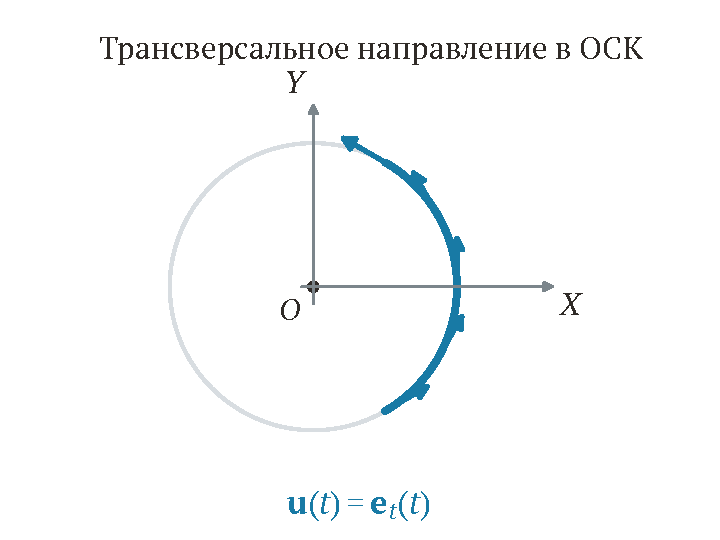
\includegraphics[width=\linewidth]{images/orientation-orbital.pdf}
\caption{Направление тяги поворачивается вместе с базисом ОСК.}
\label{fig:orientation-orbital}
\end{minipage}\hfill
\begin{minipage}[t]{.485\textwidth}
\centering
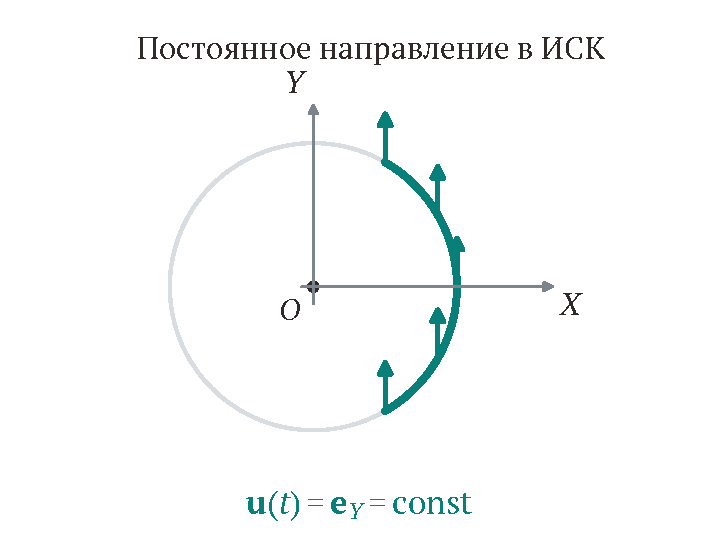
\includegraphics[width=\linewidth]{images/orientation-inertial.pdf}
\caption{Направление тяги постоянно в ИСК. Векторы тяги
в разных точках параллельны.}
\label{fig:orientation-inertial}
\end{minipage}
\end{figure}

\textit{Постоянное направление в инерциальной системе.}
Задаётся единичный вектор $\vect u_0$ с постоянными инерциальными
компонентами:
\begin{equation}
\vect u(t)=\vect u_0=\mathrm{const}.
\label{eq:inertial-direction}
\end{equation}
При этом его компоненты в текущей ОСК меняются:
$u_r=\vect u_0\cdot\vect e_r$,
$u_t=\vect u_0\cdot\vect e_t$,
$u_n=\vect u_0\cdot\vect e_n$.
Даже если в центре манёвра тяга направлена трансверсально,
в остальных точках она будет иметь и радиальную компоненту
(рисунок~\ref{fig:orientation-inertial}).

Таким образом, одинаковые модуль тяги и её направление в одной
точке ещё не задают одинаковые протяжённые манёвры. В расчёте
должен быть выбран один из законов \eqref{eq:orbital-direction},
\eqref{eq:inertial-direction}.

\subsection{Характеристическая скорость и длительность манёвра}

Импульсное решение удобно использовать как начальное приближение:
модуль рассчитанного импульса принимается за характеристическую
скорость протяжённого манёвра. Эта величина определяется интегралом
модуля управляющего ускорения:
\begin{equation}
\Delta V=\int_{t_b}^{t_e}\norm{\vect a(t)}\dd t
        =\int_{t_b}^{t_e}\frac{F(t)}{m(t)}\dd t,
\qquad \tau=t_e-t_b.
\label{eq:dv-char}
\end{equation}
Индексы $b$ и $e$ относятся к началу и концу манёвра:
$m_b=m(t_b)$, $m_e=m(t_e)$.

При постоянном $c$ уравнение расхода массы даёт
$F\dd t=-c\dd m$. После подстановки в \eqref{eq:dv-char} получаем
\begin{equation}
\Delta V=-c\int_{m_b}^{m_e}\frac{\dd m}{m}
        =c\ln\frac{m_b}{m_e},
\qquad m_e=m_b\exp(-\Delta V/c).
\label{eq:rocket}
\end{equation}
По заданной характеристической скорости определяется конечная
масса и, следовательно, расход топлива. Направление тяги
в \eqref{eq:rocket} не входит.

Характеристическую скорость следует отличать от изменения
инерциального вектора скорости. Из \eqref{eq:motion} следует
\begin{equation}
\vect V_e-\vect V_b
=\int_{t_b}^{t_e}\left(-\frac{\mu\vect R}{R^3}
                   +\vect a_{\text{возм}}\right)\dd t
 +\int_{t_b}^{t_e}\vect a(t)\dd t.
\label{eq:velocity-difference}
\end{equation}
Первый интеграл описывает действие гравитации и возмущений,
второй --- двигателя. Для второго интеграла
\[
\left\|\int_{t_b}^{t_e}\vect a(t)\dd t\right\|
\leqslant\int_{t_b}^{t_e}\norm{\vect a(t)}\dd t=\Delta V.
\]
Если инерциальное направление тяги постоянно, вклады двигателя
параллельны и равенство достигается. При повороте направления
они складываются векторно, поэтому их суммарный модуль может
быть меньше. В обоих случаях полный вектор
$\vect V_e-\vect V_b$ содержит также первый интеграл
\eqref{eq:velocity-difference}; его модуль не определяется
одной характеристической скоростью.

При постоянной тяге $F>0$ масса изменяется по закону
$m(t)=m_b-(F/c)(t-t_b)$. Время, необходимое для расходования
$m_b-m_e$, равно
\begin{equation}
\boxed{\displaystyle
\tau=\frac{c(m_b-m_e)}{F}
    =\frac{m_bc}{F}\left(1-e^{-\Delta V/c}\right).}
\label{eq:duration}
\end{equation}
Если $\Delta V/c\ll1$, разложение экспоненты даёт
$\tau\simeq m_b\Delta V/F$.
Точная формула учитывает возрастание ускорения во время манёвра
и даёт меньшую длительность, чем эта оценка с начальной массой.

\begin{explanation}{От заданной характеристической скорости к длительности}
При известных $m_b$, $F$ и $I_{\mathrm{sp}}$ рассчитанная в импульсной
модели величина $\Delta V$ задаёт расход топлива по
\eqref{eq:rocket} и длительность $\tau$ по \eqref{eq:duration}.
Полученные $\tau$ и закон направления тяги используются
в уравнениях движения. Результат этого прогноза показывает,
какую орбиту создаёт выбранный протяжённый манёвр.
\end{explanation}

\subsection{Изменение энергии и орбитального момента}

Почему равенство характеристических скоростей не сохраняет
конечную орбиту? Для ответа удобно проследить два механических
параметра: удельную энергию
$\mathcal E=V^2/2-\mu/R$ и удельный орбитальный момент
$\vect h=\vect R\times\vect V$.
Дифференцирование с учётом \eqref{eq:motion} даёт
\begin{equation}
\dot{\mathcal E}=\vect V\cdot\vect a_{\text{возм}}
 +\frac{F}{m}\vect V\cdot\vect u,\qquad
\dot{\vect h}=\vect R\times\vect a_{\text{возм}}
 +\frac{F}{m}\vect R\times\vect u.
\label{eq:energy-momentum}
\end{equation}
Центральное ускорение сокращается с производной потенциала
в первом равенстве и имеет нулевой момент во втором.
Изменение энергии зависит от текущей скорости,
изменение момента --- от текущего положения и направления тяги.

Для импульса $\Delta\vect V$ точные изменения этих параметров
выражаются формулами
\begin{equation}
\Delta\mathcal E=\vect V^-\cdot\Delta\vect V
 +\frac{\norm{\Delta\vect V}^2}{2},\qquad
\Delta\vect h=\vect R\times\Delta\vect V.
\label{eq:impulse-invariants}
\end{equation}
При одинаковом $\Delta V=\norm{\Delta\vect V}$ наибольшее
увеличение энергии в данной точке достигается импульсом вдоль
скорости. На одной эллиптической орбите скорость максимальна
в перицентре, поэтому такой импульс даёт там наибольшее
$\Delta\mathcal E=V\Delta V+\Delta V^2/2$.

Для увеличения \emph{модуля орбитального момента} выгодно другое
положение. Если импульс трансверсален и направлен по движению,
то $\Delta\vect h$ параллелен исходному $\vect h$ и
\[
\Delta h=R\Delta V.
\]
При одинаковом $\Delta V$ изменение $h$ максимально в апоцентре,
где плечо $R$ наибольшее. В апсидах скорость трансверсальна,
поэтому сравниваются импульсы одного направления относительно
локального движения, но с разным механическим результатом.

Энергия и момент совместно определяют размеры и форму
оскулирующей орбиты:
\[
a=-\frac{\mu}{2\mathcal E},\qquad
e^2=1+\frac{2\mathcal E h^2}{\mu^2}.
\]
Требование увеличить энергию выделяет перицентр, а требование
увеличить момент трансверсальным импульсом --- апоцентр.
Выбор места манёвра зависит от того, какие изменения $a$ и $e$
нужны одновременно. При протяжённом манёвре значения
$\vect R$ и $\vect V$ меняются внутри участка, поэтому
\eqref{eq:energy-momentum} интегрируется вдоль траектории.
Это связывает закон направления тяги и размещение манёвра
с конечной орбитой; одна величина $\Delta V$ эту связь не задаёт.

\FloatBarrier
\section{Размещение протяжённого манёвра относительно импульса}
\label{sec:placement}

После определения длительности остаётся выбрать начало манёвра.
Если весь манёвр выполняется после момента рассчитанного импульса,
воздействие систематически смещается вперёд по времени.
Центрирование относительно этого момента уменьшает такое смещение.
Далее покажем, какой член ошибки устраняется симметрией и при
каких предположениях справедлив этот вывод.

\subsection{Начало, центр и угловая протяжённость манёвра}

Обозначим момент исходного импульса через $t_{\mathrm{imp}}$,
а центр протяжённого манёвра --- через
$t_c=(t_b+t_e)/2$. При центрировании $t_c=t_{\mathrm{imp}}$, то есть
\begin{equation}
t_b=t_{\mathrm{imp}}-\frac\tau2,\qquad
t_e=t_{\mathrm{imp}}+\frac\tau2.
\label{eq:centering}
\end{equation}
Начало манёвра в точке импульса означает другой выбор:
\begin{equation}
t_b=t_{\mathrm{imp}},\qquad
t_e=t_{\mathrm{imp}}+\tau,\qquad
t_c=t_{\mathrm{imp}}+\frac\tau2.
\label{eq:start-at-impulse}
\end{equation}
Во втором случае центр смещён на $\tau/2$.
При заданном конечном моменте $t_f$ это меняет не только
положение КА во время манёвра, но и время пассивного движения
после его завершения. Поэтому варианты сравниваются
при одном и том же $t_f$.

Для представления геометрического масштаба участка полезна
его угловая протяжённость. На опорной кеплеровской орбите
истинная аномалия изменяется со скоростью $h/R^2$, поэтому
\begin{equation}
\theta=\nu(t_e)-\nu(t_b)
      =\int_{t_b}^{t_e}\frac{h}{R(t)^2}\dd t,
\qquad h=\norm{\vect R\times\vect V}.
\label{eq:arc}
\end{equation}
Разность аномалий здесь вычисляется без приведения к одному
обороту. Эта оценка показывает, насколько различаются положения,
в которых распределено воздействие. На эллиптической орбите
одна и та же длительность соответствует большему $\theta$
около перицентра и меньшему --- около апоцентра.
Поэтому отношение $\tau$ к периоду недостаточно характеризует
локальность манёвра. Для круговой опорной орбиты
\eqref{eq:arc} упрощается до $\theta=n_0\tau$;
эта связь понадобится в следующей главе.

\subsection{Почему центрирование уменьшает ошибку приближения}

В предыдущей лекции вводилась матрица манёвра
$M(t)=\Phi(t_f,t)B(t)$.
Матрица $B(t)$ связывает управляющее ускорение с изменением
выбранных переменных движения, а $\Phi(t_f,t)$ переносит
малое отклонение из момента $t$ в общий конечный момент $t_f$.
При малом управлении изменение конечного состояния в первом
порядке имеет вид
\begin{equation}
\delta\vect y_f=\int_{t_b}^{t_e}M(t)\vect a(t)\dd t.
\label{eq:duhamel}
\end{equation}
Каждый элемент $M(t)$ описывает, как малая составляющая
управления в момент $t$ влияет на соответствующую конечную
переменную. Если эта чувствительность заметно меняется
в течение манёвра, распределение воздействия по времени
нельзя заменить одним интегралом модуля ускорения.

В \eqref{eq:duhamel} используется линеаризация около выбранной
опорной траектории: по её положениям и скоростям вычисляются
коэффициенты $B$ и $\Phi$. Если опорная траектория пассивна,
$\vect a$ означает добавляемое управляющее ускорение.
Возможна и линеаризация около уже рассчитанного движения
с тягой: тогда в правой части стоит малое изменение ускорения,
а матрицы определяются для этого движения. При последовательном
уточнении опорную траекторию и матрицы можно рассчитывать заново.
Следовательно, вычисление вдоль опорной траектории является
основой локального линейного приближения, а не требованием
использовать только пассивную или круговую орбиту.

Рассмотрим постоянный по времени столбец ускорения
$\vect a=\Delta\vect V/\tau$.
Компоненты ускорения и столбцы $B(t)$ должны относиться
к одной системе координат. Для инерциальных компонент
$\Delta\vect V$ --- постоянный инерциальный вектор;
для постоянных компонент в ОСК её поворот включается в $B(t)$.
При центрировании получаем
\begin{equation}
\delta\vect y_f=\overline M\Delta\vect V,\qquad
\overline M=\frac1\tau
\int_{t_c-\tau/2}^{t_c+\tau/2}M(t)\dd t.
\label{eq:average-M}
\end{equation}
Импульс в центре дал бы $M(t_c)\Delta\vect V$.
Чтобы найти разность, положим $s=t-t_c$ и разложим гладкую
матрицу по Тейлору:
\begin{equation}
M(t_c+s)=M(t_c)+s\dot M(t_c)
 +\frac{s^2}{2}\ddot M(t_c)
 +\frac{s^3}{6}M^{(3)}(t_c)+O(s^4).
\label{eq:matrix-taylor}
\end{equation}
Для симметричного интервала
\[
\int_{-\tau/2}^{\tau/2}\dd s=\tau,\qquad
\int_{-\tau/2}^{\tau/2}s\dd s=0,\qquad
\int_{-\tau/2}^{\tau/2}s^2\dd s=\frac{\tau^3}{12},\qquad
\int_{-\tau/2}^{\tau/2}s^3\dd s=0.
\]
Подставляя \eqref{eq:matrix-taylor} в \eqref{eq:average-M}, находим
\begin{equation}
\begin{aligned}
\overline M
&=\frac1\tau\left[
 \tau M(t_c)+0\,\dot M(t_c)
 +\frac12\frac{\tau^3}{12}\ddot M(t_c)
 +O(\tau^5)\right]\\
&=M(t_c)+\frac{\tau^2}{24}\ddot M(t_c)+O(\tau^4).
\end{aligned}
\label{eq:midpoint-error}
\end{equation}
Линейный по времени член исчезает: вклады до и после центра
имеют противоположные знаки. Первый сохраняющийся член
разности $\overline M-M(t_c)$ пропорционален $\tau^2$.

Если манёвр \emph{начинается} в момент импульса, интегрирование
выполняется по $0\leqslant s\leqslant\tau$:
\begin{equation}
\frac1\tau\int_{t_{\mathrm{imp}}}^{t_{\mathrm{imp}}+\tau}M(t)\dd t
=M(t_{\mathrm{imp}})
 +\frac\tau2\dot M(t_{\mathrm{imp}})
 +\frac{\tau^2}{6}\ddot M(t_{\mathrm{imp}})+O(\tau^3).
\label{eq:start-error}
\end{equation}
Здесь сохраняется член $\tau\dot M/2$.
При постоянных компонентах ускорения и коротком участке
центрирование \eqref{eq:centering} поэтому даёт более точное
приближение исходного импульса, чем размещение
\eqref{eq:start-at-impulse}: ошибка усреднения начинается
со второго порядка по длительности вместо первого.

Для переменного модуля ускорения при неизменном направлении
в выбранной системе компонент вклад разных моментов имеет
разные веса. Это может быть инерциальная система или ОСК;
используемый базис учитывается в $B(t)$. Положим
$w(t)=\norm{\vect a(t)}/\Delta V$, так что
$\int_{t_b}^{t_e}w(t)\dd t=1$, и определим среднее время
приложения воздействия
\[
\overline t=\int_{t_b}^{t_e}t\,w(t)\dd t.
\]
Член с первой производной матрицы теперь равен
$\dot M(t_c)(\overline t-t_c)\Delta\vect V$.
Он исчезает, если профиль ускорения симметричен относительно
$t_c$. При постоянной тяге и заметном расходе массы ускорение
возрастает, поэтому одной симметрии границ по времени
для точного сокращения этого члена недостаточно.

\subsection{Что определяет применимость импульсного приближения}

В рассмотренном выводе используются два разных приближения.
Первое --- линеаризация движения по малому управляющему
воздействию. Отношение $\Delta V/V$ характеризует относительный
масштаб изменения скорости; малость изменений выбранных
элементов орбиты оценивается дополнительно.
Второе --- замена распределённого управления импульсом,
основанная на малом изменении $M(t)$ за время манёвра.

Эти условия не совпадают. Малый по характеристической скорости
манёвр при малой тяге может занимать значительную часть витка;
тогда линейная теория ещё описывает изменение орбиты,
но матрица в одной точке уже недостаточно представляет
интеграл \eqref{eq:duhamel}.
Центрирование устраняет первый член ошибки размещения,
а оставшийся результат зависит от изменения чувствительностей
в течение участка. Это и требуется учитывать при переходе
от импульсной модели к модели с конечной тягой.

\FloatBarrier
\section{Влияние направления тяги: пример около круговой орбиты}
\label{sec:circular}

На круговой опорной орбите можно явно вычислить, как распределение
одной характеристической скорости меняет большую полуось
и эксцентриситет. Такое сопоставление показывает физический смысл
двух законов ориентации из пункта~1.2 и позволяет отделить
изменение энергии от изменения формы орбиты.

\subsection{Два закона направления и их орбитальный результат}

Рассмотрим плоский манёвр около круговой орбиты радиуса $r_0$.
Её скорость и среднее движение равны
$V_0=\sqrt{\mu/r_0}$, $n_0=\sqrt{\mu/r_0^3}$.
Инерциальная ось $X$ направлена по радиусу опорной орбиты
в центре манёвра, ось $Y$ --- по орбитальной скорости
в этой точке. Угол $\varphi=n_0(t-t_c)$ изменяется
от $-\theta/2$ до $\theta/2$, где $\theta=n_0\tau$.
В этом примере модуль ускорения постоянен:
$A=\Delta V/\tau$; расход массы не моделируется.

Околокруговое приближение здесь означает сохранение членов
первого порядка по $\varepsilon=\Delta V/V_0\ll1$.
Приращения $a-r_0$, $e_x$, $e_y$ вычисляются линейно
по управлению, а положение и скорость в их коэффициентах
берутся на опорной круговой орбите. Члены порядка
$\varepsilon^2$ отбрасываются при фиксированном $\theta$.
Малость $\theta$ для следующих формул не требуется.
Это приближение не используется при расчёте перехода
между эллиптическими орбитами в главе~\ref{sec:example}.

Пусть $S$ и $T$ --- радиальная и трансверсальная компоненты
управляющего ускорения. Из изменения энергии
$\dot{\mathcal E}=V_0T$ в первом порядке следует
$\dot a=2r_0T/V_0$.
Для вектора эксцентриситета дифференцирование
$\vect e=(\vect V\times\vect h)/\mu-\vect R/R$ даёт
\[
\dot{\vect e}
=\frac{\vect a\times\vect h+
        \vect V\times(\vect R\times\vect a)}{\mu}
=\frac{2T\vect e_r-S\vect e_t}{V_0}
\]
после подстановки опорного кругового движения. Записывая базис
в неподвижных осях,
\[
\vect e_r=(\cos\varphi,\sin\varphi)^\top,\qquad
\vect e_t=(-\sin\varphi,\cos\varphi)^\top,
\]
получаем
\begin{equation}
\begin{aligned}
\delta a&=\frac{2r_0}{V_0}\int_{t_b}^{t_e}T\dd t,\\
\delta e_x&=\frac1{V_0}\int_{t_b}^{t_e}
       (S\sin\varphi+2T\cos\varphi)\dd t,\\
\delta e_y&=\frac1{V_0}\int_{t_b}^{t_e}
       (-S\cos\varphi+2T\sin\varphi)\dd t.
\end{aligned}
\label{eq:circle-integrals}
\end{equation}
Компоненты $e_x,e_y$ определены в одних и тех же неподвижных
осях $X,Y$. Поскольку исходная орбита круговая,
её вектор эксцентриситета равен нулю и конечные компоненты
в первом порядке равны $\delta e_x,\delta e_y$.

\textit{1. Направление постоянно в ОСК и трансверсально.}
В соответствии с первым способом из пункта~1.2
$\vect a=A\vect e_t(t)$, поэтому $S=0$, $T=A$.
В каждой точке изменение вектора эксцентриситета направлено
по текущему радиусу: $\dot{\vect e}=(2A/V_0)\vect e_r$.
Симметричные относительно $X$ вклады имеют противоположные
проекции на $Y$ и одинаковые проекции на $X$
(рисунок~\ref{fig:circle-orbital}).

\coursefigure{circle-orbital}{Трансверсальное ускорение
на круговой опорной орбите. Справа показаны вклады
$\dot{\vect e}$ в двух симметричных положениях
$\pm\varphi$ за одинаковые малые промежутки времени.
Их поперечные составляющие сокращаются, а составляющие вдоль
$X$ складываются.}

Замена $\dd t=\dd\varphi/n_0$ даёт
\[
\delta e_x=\frac{2A}{n_0V_0}
 \int_{-\theta/2}^{\theta/2}\cos\varphi\dd\varphi
=\frac{4A}{n_0V_0}\sin\frac\theta2.
\]
Поскольку $A\tau=\Delta V$ и $n_0\tau=\theta$,
\begin{equation}
\boxed{\displaystyle
\delta a=\frac{2r_0\Delta V}{V_0},\qquad
\delta e_x=\frac{2\Delta V}{V_0}\sinc\frac\theta2,
\qquad \delta e_y=0,}
\label{eq:circle-rtn}
\end{equation}
где $\sinc x=\sin x/x$ при $x\ne0$, $\sinc0=1$.
Изменение полуоси не зависит от $\theta$ при фиксированном
$\Delta V$: в первом порядке скорость всюду равна $V_0$,
а ускорение направлено вдоль неё. Изменение эксцентриситета
уменьшается с ростом $\theta$, поскольку направления
частных вкладов $\dot{\vect e}$ всё сильнее различаются.

\textit{2. Направление постоянно в инерциальной системе.}
Зафиксируем направление тяги вдоль неподвижной оси $Y$:
$\vect a=A\vect e_Y$. Это второй способ из пункта~1.2;
в центре манёвра направление совпадает с трансверсальным.
В остальных точках
\[
S=A\sin\varphi,\qquad T=A\cos\varphi.
\]
Поэтому подынтегральные выражения для эксцентриситета имеют вид
\[
S\sin\varphi+2T\cos\varphi
=A(\sin^2\varphi+2\cos^2\varphi)
=A\left(\frac32+\frac12\cos2\varphi\right),
\]
\[
-S\cos\varphi+2T\sin\varphi
=A\sin\varphi\cos\varphi.
\]
Второе выражение нечётно, поэтому $\delta e_y=0$.
Первое положительно на всём участке: радиальная составляющая
ускорения также участвует в изменении $e_x$.

\coursefigure{circle-inertial}{Постоянное ускорение вдоль
инерциальной оси $Y$. Орбитальные компоненты $S$ и $T$ меняются
с положением КА. Справа симметричные вклады в вектор
эксцентриситета сопоставлены с рисунком~\ref{fig:circle-orbital}:
направление суммы то же, но проекции отдельных вкладов отличаются.}

Интегрируя \eqref{eq:circle-integrals}, получаем
\begin{equation}
\boxed{\displaystyle
\delta a=\frac{2r_0\Delta V}{V_0}\sinc\frac\theta2,\qquad
\delta e_x=\frac{2\Delta V}{V_0}
 \left(\frac34+\frac14\sinc\theta\right),\qquad
\delta e_y=0.}
\label{eq:circle-inertial}
\end{equation}
Теперь увеличение полуоси уменьшается: на краях участка
трансверсальная составляющая $A\cos\varphi$ меньше $A$.
При этом изменение эксцентриситета не имеет того же
коэффициента, что и изменение полуоси.

Для количественного сравнения введём коэффициенты
\begin{equation}
k_a=\frac{\delta a}{2r_0\Delta V/V_0},\qquad
k_e=\frac{\delta e_x}{2\Delta V/V_0}.
\label{eq:circle-coefficients}
\end{equation}
Знаменатели --- изменения от трансверсального импульса
в центре участка в первом порядке.
Для $0\leqslant\theta\leqslant180^\circ$ в обоих случаях
$\delta e_x\geqslant0$, $\delta e_y=0$, поэтому $k_e$ одновременно
характеризует изменение модуля эксцентриситета.
Зависимости \eqref{eq:circle-rtn}, \eqref{eq:circle-inertial}
получены у Баранова \cite[§6.1.1, §6.1.3]{baranov}
и показаны на рис.~\ref{fig:circular-response}.

\coursefigure{circular-response}{Зависимость коэффициентов
$k_a$ и $k_e$ от угловой протяжённости манёвра.
Линии рассчитаны по \eqref{eq:circle-rtn},
\eqref{eq:circle-inertial}. Точки соответствуют нелинейному
расчёту из пункта~3.2. При $\theta\to0$ оба закона
дают импульсный результат первого порядка.}

При $\theta=180^\circ$ трансверсальная ориентация даёт
$k_a=1$, $k_e=2/\pi\simeq0.637$;
инерциальная --- $k_a=2/\pi$, $k_e=0.75$.
Если требуется увеличить полуось, первый закон эффективнее
в рассмотренном приближении. Если сравнивается только увеличение
эксцентриситета, второй закон при той же протяжённости даёт
больший результат. Таким образом, эффективность относится
к выбранному изменению орбиты. Единого коэффициента,
которым можно умножить $\Delta V$ для получения всех
эффектов протяжённого манёвра, здесь нет.

\subsection{Численная проверка}

Возьмём $r_0=\CircRadius$~км и $\Delta V=\CircDVMps$~м/с.
Скорость опорной круговой орбиты равна $\CircVelocity$~км/с,
период --- $\CircPeriodMinutes$~мин,
$\Delta V/V_0\simeq1.33\cdot10^{-4}$.
Для каждого $\theta$ начальное состояние в $t_b$
берётся на опорной круговой орбите. Затем интегрируются
нелинейные уравнения движения в центральном поле
с постоянным модулем ускорения $A=\Delta V/\tau$
и одним из двух законов направления. При ориентации в ОСК
её базис определяется по текущему состоянию КА.

Для $\theta=180^\circ$ длительность равна
$\CircHalfOrbitMinutes$~мин. Получаем
\begin{center}
\renewcommand{\arraystretch}{1.15}
\begin{tabular}{@{}lrrrr@{}}
\toprule
&\multicolumn{2}{c}{$\delta a$, м}
&\multicolumn{2}{c}{$e_x\cdot10^4$}\\
Направление&Линейно&Нелинейно&Линейно&Нелинейно\\\midrule
В текущей ОСК&1855{,}274&1855{,}743&1{,}687292&1{,}687572\\
В инерциальной системе&1181{,}104&1181{,}403&1{,}987794&1{,}987878\\
\bottomrule
\end{tabular}
\end{center}
На проверенном диапазоне $1$--$180^\circ$ разность линейного
и нелинейного результатов по полуоси не превышает $0.615$~м.
Для вектора эксцентриситета
$r_0\norm{\vect e_{\text{нелин}}-\vect e_{\text{лин}}}<0.197$~м;
в эту разность входит и малая компонента $e_y$
нелинейного решения. Ужесточение допусков и уменьшение
максимального шага меняют результаты менее чем на
$3\cdot10^{-8}$~м в этих двух мерах.

При выбранном малом $\Delta V/V_0$ численный расчёт подтверждает
полученное различие двух законов направления даже для участка
в половину витка. Длительность сама по себе не задаёт ошибку
импульсного приближения: требуется учитывать, какая величина
изменяется и как направлена тяга. В последующем расчёте последовательности манёвров используются
уравнения Гаусса с расходом массы.

\FloatBarrier
\FloatBarrier
\section{Последовательность протяжённых манёвров}
\label{sec:sequence}

Замена импульса одним протяжённым манёвром может потребовать
слишком долгой работы двигателя: за это время положение КА
и орбитальный эффект тяги существенно изменяются. Один из способов
приблизиться к исходному импульсному решению --- распределить
его характеристическую скорость между несколькими манёврами
на разных витках. Каждый из них короче, а между ними можно
определить достигнутую орбиту и пересчитать оставшуюся часть перехода.
Для построения такой последовательности нужно выбрать доли
характеристической скорости, положения манёвров и направления тяги.

\subsection{Распределение характеристической скорости с помощью весов}

Номинальная последовательность определяется начальной эпохой,
начальными орбитальными элементами, массой $m_0$ и упорядоченным набором
манёвров. Для каждого задаются начало $t_{b,j}$, длительность
$\tau_j$, тяга, $I_{\mathrm{sp}}$ и закон направления тяги.
Если задана характеристическая скорость $\Delta V_j$, длительность
определяется по массе в начале манёвра из \eqref{eq:duration}.
Дополнительно выбираются модель возмущений и конечная эпоха прогноза.

Рассмотрим группу из $N$ манёвров, заменяющую один исходный
импульсный манёвр. Веса $w_j$ задают доли его характеристической скорости:
\begin{equation}
\Delta V_j=w_j\Delta V_{\text{гр}},\qquad
w_j\geqslant0,\qquad \sum_{j=1}^{N}w_j=1.
\label{eq:weights}
\end{equation}
Сумма $\Delta V_j$ сохраняется, но положения манёвров и направления
тяги ещё предстоит назначить. Именно от них зависит, насколько
полученная последовательность приблизит КА к нужной орбите.

При постоянных $F$ и $c$ массы и длительности связаны равенствами
\begin{equation}
\begin{aligned}
m_{e,j}&=m_{b,j}\exp\!\left(-\frac{w_j\Delta V_{\text{гр}}}{c}\right),\\
\tau_j&=\frac{c\,m_{b,j}}{F}
 \left[1-\exp\!\left(-\frac{w_j\Delta V_{\text{гр}}}{c}\right)\right].
\end{aligned}
\label{eq:weighted-time}
\end{equation}
На пассивном участке расход топлива отсутствует, поэтому
$m_{b,j+1}=m_{e,j}$. Равные веса означают равные $\Delta V_j$,
но длительности таких манёвров уменьшаются по мере расхода топлива.
Если же поровну распределять время работы двигателя, то расход массы
в каждом манёвре одинаков, а $\Delta V_j$ возрастает.
Поэтому вместе с весами всегда нужно указывать, какая величина распределяется.

\subsection{Перенос положения и направления на другие витки}

Чтобы повторять манёвр на следующих витках, необходимо определить,
что означает «в том же месте». Например, если исходный импульс
рассчитан в перицентре, центры манёвров группы можно располагать
около перицентров последующих орбит. Если важнее направление
радиуса в инерциальном пространстве, фиксируют именно это направление.
Эти два подхода совпадают только пока линия апсид сохраняет положение.

Аналогичный выбор требуется для направления тяги.
Можно сохранять инерциальное направление исходного импульса
либо его компоненты относительно местной ОСК в центре каждого
следующего манёвра. В первом случае КА воспроизводит направление
в пространстве; во втором --- ориентацию относительно текущей орбиты.
Для начального построения выбирают вариант, соответствующий
назначению манёвра: изменению размера, формы или плоскости орбиты.
Последствия этого выбора при возмущённом движении рассмотрим
в разделе~\ref{sec:perturbations}.

\subsection{Ошибки исполнения и смысл дробления манёвра}
\label{sec:errors}

Рассчитанные величина и направление манёвра известны заранее,
а фактически сообщённое воздействие определяется после его исполнения.
Они различаются из-за неточного знания тяги, длительности работы
двигателя и ориентации КА. Сначала рассмотрим ошибку величины
характеристической скорости, сохраняя запланированное направление.
Относительная ошибка определяется как
\begin{equation}
\delta_j=
\frac{\Delta V_{j,\text{факт}}-\Delta V_{j,\text{план}}}
     {\Delta V_{j,\text{план}}},\qquad
\Delta V_{j,\text{факт}}=(1+\delta_j)\Delta V_{j,\text{план}}.
\label{eq:relative-error}
\end{equation}
Например, $\delta_j=0.01$ означает превышение запланированной
величины на $1\%$. Абсолютная ошибка равна
$\delta_j\Delta V_{j,\text{план}}$: при одной относительной
ошибке она меньше у меньшего манёвра.
Ошибкой направления называется отклонение фактического направления
от запланированного; уменьшение величины манёвра также уменьшает
модуль вызванной этим векторной ошибки при одинаковом угле отклонения.

Систематическая ошибка имеет общую причину и воспроизводится
в нескольких манёврах. Пусть во всех манёврах группы одна и та же
неустранённая ошибка величины $\delta_{\text{сист}}$.
Тогда независимо от выбранных весов
\begin{equation}
\begin{aligned}
\sum_j\Delta V_{j,\text{факт}}
&=\sum_j(1+\delta_{\text{сист}})\Delta V_{j,\text{план}}\\
&=(1+\delta_{\text{сист}})\Delta V_{\text{гр}}.
\end{aligned}
\label{eq:systematic}
\end{equation}
Дробление само по себе не устраняет такую ошибку.
Преимущество последовательности появляется, если по результату
первых манёвров удаётся оценить отклонение и изменить последующие
манёвры, в том числе уточнить используемую модель двигателя.

\subsection{Равные и убывающие веса: разные цели выбора}

Теперь сравним два способа задания весов из \eqref{eq:weights}.
\textit{При равном распределении} $w_j=1/N$ все манёвры имеют
характеристическую скорость $\Delta V_{\text{гр}}/N$.
Для любого другого распределения
\begin{equation}
\max_j\Delta V_j\geqslant
\frac{1}{N}\sum_j\Delta V_j=
\frac{\Delta V_{\text{гр}}}{N}.
\label{eq:equal-minmax}
\end{equation}
Следовательно, равные веса минимизируют наибольшую величину
отдельного манёвра при заданных сумме и числе манёвров.
Это полезно, когда важно избежать большого распределённого воздействия
вдалеке от выбранного орбитального положения. Полученный результат
относится к $\Delta V_j$; длительности зависят также от текущей массы,
а пройденные углы --- от скорости движения по орбите.

\textit{При убывающем распределении} большая часть изменения орбиты
выполняется раньше, а заключительный манёвр мал.
Например, можно взять веса, пропорциональные
$1,k,k^2,\ldots,k^{N-1}$, где $0<k<1$, и нормировать их сумму к единице.
При относительной модели \eqref{eq:relative-error} уменьшение
последнего манёвра уменьшает и его абсолютную ошибку.
Это важно именно в конце перехода: после заключительного манёвра
в первоначальной последовательности уже нет средств для исправления
его результата.

Такой выбор требует заранее оценить возможности оставшейся части
последовательности. После большого раннего манёвра должно оставаться
достаточно характеристической скорости и свободы выбора направления,
чтобы исправить ожидаемое отклонение. Если сделать только последний
манёвр чрезвычайно малым, ошибка предпоследнего может оказаться
больше доступной коррекции. Поэтому размеры уменьшают постепенно,
а после измерения достигнутой орбиты оставшиеся величины пересчитывают.
Убывающие веса дают способ организовать завершение перехода,
но не увеличивают располагаемый запас топлива.

\subsection{Использование последующих манёвров для коррекции}

Поскольку манёвры исполняются с ошибками, оставшуюся часть
последовательности полезно пересчитывать по достигнутому состоянию.
Это позволяет исправлять последствия предшествующих манёвров
в процессе выполнения самого перехода.
Рассмотрим сначала простую векторную схему: все изменения скорости
относятся к одной точке и к одной системе координат.
Если вместо $\Delta\vect V_1$ получено
$\Delta\vect V_1+\vect\varepsilon$, то для сохранения заданной
суммы оставшееся воздействие должно измениться с
$\Delta\vect V_{\text{ост}}$ на
$\Delta\vect V_{\text{ост}}-\vect\varepsilon$.

Например, запланированы два сонаправленных манёвра:
100 и 20~м/с. Если первый сообщил 99~м/с, то после определения
этой ошибки второй можно пересчитать на 21~м/с.
Цель $120$~м/с достигается без дополнительного манёвра
и с той же суммарной характеристической скоростью.
Если же последний манёвр должен был сообщить 120~м/с,
но сообщил 121~м/с, потребуется отдельный манёвр 1~м/с
в противоположном направлении. Сумма модулей воздействий
тогда составит 122~м/с (рис.~\ref{fig:error-compensation}).

\coursefigure{error-compensation}{Коррекция в одномерной схеме
сложения приращений скорости. Слева ошибку первого манёвра
компенсирует пересчитанный второй манёвр. Справа показано
увеличение области около цели: после избыточного последнего
манёвра требуется обратное воздействие. Орбитальное движение
между манёврами в этой иллюстрации не рассматривается.}

Условие полезности коррекции --- возможность оценить фактический
результат и изменить последующие манёвры. Очень малый последний
манёвр не обеспечивает исправления любого прежнего отклонения:
имеют значение величина и допустимое направление требуемой коррекции.
При движении по орбите последующие манёвры рассчитываются
из фактически достигнутого состояния, а целью остаётся
заданная конечная орбита.

\subsection{Последовательный прогноз}

После назначения параметров все манёвры рассчитываются
в составе одной траектории. Это необходимо, поскольку каждый
предыдущий манёвр изменяет начальные условия последующего.
При заданных временах прогноз выполняется так:
\begin{enumerate}
\item Рассчитать пассивное движение от исходного состояния
до начала первого манёвра $t_{b,1}$.
\item Интегрировать уравнения движения с тягой до
$t_{e,1}=t_{b,1}+\tau_1$.
\item Использовать полученные орбитальные элементы и массу как
начальные данные следующего пассивного участка.
\item Повторить расчёт пассивного участка и манёвра
для всей последовательности.
\item После последнего манёвра продолжить прогноз до $t_f$
и определить, достигнуты ли заданные конечные условия.
\end{enumerate}

\begin{figure}[htbp]
\centering
\begin{tikzpicture}[x=1cm,y=1cm,>=Latex,font=\small]
\draw[->,figink] (0,0)--(15,0) node[right] {$t$};
\foreach \l/\r/\name in {2/4/1,7/8.4/2,11.7/12.5/3}{
 \fill[accent!18] (\l,.15) rectangle (\r,1.15);
 \draw[accent,thick] (\l,.15)--(\l,1.15)--(\r,1.15)--(\r,.15);
 \node[accent] at ({(\l+\r)/2},1.43) {манёвр \name};
 \draw[densely dashed,muted] (\l,0)--(\l,1.2);
 \draw[densely dashed,muted] (\r,0)--(\r,1.2);
}
\node[muted] at (1,.55) {прогноз};
\node[muted] at (5.5,.55) {пауза};
\node[muted] at (10,.55) {пауза};
\node[muted] at (13.7,.55) {прогноз};
\node[below] at (0,0) {$t_0$};
\node[below] at (2,0) {$t_{b,1}$};
\node[below] at (4,0) {$t_{e,1}$};
\node[below] at (14.7,0) {$t_f$};
\draw[<->,accent] (2,-.7)--node[below] {$\tau_1$}(4,-.7);
\draw[<->,muted] (4,-.7)--node[below] {$\Delta t_1$}(7,-.7);
\end{tikzpicture}
\caption{Последовательность манёвров и пассивных участков.
Результат каждого участка становится начальным условием следующего.}
\label{fig:timeline}
\end{figure}

\FloatBarrier
\section{Возмущения и перенос геометрии манёвров}
\label{sec:perturbations}

В центральном поле ориентация орбиты на пассивном участке
сохраняется. В реальном движении орбита меняется и между манёврами.
Поэтому последовательность, построенная повторением исходной
геометрии на следующих витках, может дать другой результат.
Нужно понять, какие положения и направления следует переносить
вместе с орбитой, а какие должны оставаться фиксированными
в инерциальном пространстве.

\subsection{Как меняются место манёвра и направление тяги}

Нецентральность гравитационного поля Земли, прежде всего $J_2$,
вызывает прецессию линии узлов и линии апсид.
Перицентр следующего витка оказывается в другом инерциальном
направлении. Если манёвр предназначен для эффективного изменения
энергии около перицентра, его положение следует выбирать
по изменившейся орбите. Фиксация прежнего инерциального
направления радиуса решает уже другую задачу.

При повороте орбитальной плоскости меняется также ОСК
в месте манёвра. Постоянный инерциальный вектор тяги получает
новые радиальную, трансверсальную и нормальную компоненты.
Например, направление, которое раньше было трансверсальным,
может теперь частично изменять плоскость орбиты.
И наоборот, сохранение нужных компонент в ОСК потребует
изменить инерциальное направление тяги
(рис.~\ref{fig:perturbed-geometry}, слева).

Обозначим через
\begin{equation}
Q_j=\begin{pmatrix}\vect e_{r,j}&\vect e_{t,j}&\vect e_{n,j}\end{pmatrix}
\label{eq:transport-basis}
\end{equation}
базис ОСК в выбранном центре $j$-го манёвра.
Если исходное инерциальное направление равно $\vect u_1$,
то его компоненты в исходной ОСК равны $\vect d=Q_1^\top\vect u_1$.
Два варианта переноса записываются как
\begin{equation}
\begin{aligned}
\text{сохранение направления в ИСК:}\quad&\vect u_j=\vect u_1,\\
\text{сохранение компонент в ОСК центра:}\quad&\vect u_j=Q_j\vect d.
\end{aligned}
\label{eq:direction-transport}
\end{equation}
Во втором варианте нужно заново рассчитать положение и скорость
у центра манёвра и построить по ним $Q_j$.
Сам вектор $\vect u_j$ после такого выбора можно считать
постоянным во время манёвра. Это перенос направления
между манёврами; непрерывная ориентация по текущей ОСК
во время манёвра представляет собой отдельный закон управления.

Сопротивление атмосферы, притяжение Солнца и Луны,
давление солнечного излучения также изменяют траекторию.
Изменения размера и формы орбиты сдвигают время достижения
нужного положения; изменения её ориентации меняют
разложение тяги на местные компоненты.
Поэтому в прогнозе выбранные возмущающие силы учитывают
как во время манёвров, так и на пассивных участках.
Перенос через ОСК сохраняет часть желаемой геометрии,
но величины и положения манёвров после этого всё равно
проверяются по достигнутой орбите.

\subsection{Оскулирующие и средние элементы}

Чтобы оценить результат переноса, необходимо определить,
какие элементы орбиты сравниваются.
\textit{Оскулирующие элементы} --- элементы кеплеровой орбиты,
которая в рассматриваемый момент имеет те же положение и скорость,
что и реальная траектория. Они соответствуют текущим положению и скорости КА
и изменяются при возмущённом движении.

В этих изменениях сочетаются быстрые колебания, связанные
с движением по орбите, и медленная эволюция.
\textit{Средние элементы} получают после исключения выбранных
периодических составляющих по определённой модели усреднения.
Они показывают медленную эволюцию орбиты, например среднюю
прецессию линии узлов. Различие между двумя представлениями
схематически показано справа на рис.~\ref{fig:perturbed-geometry}.

\begin{figure}[H]
\centering
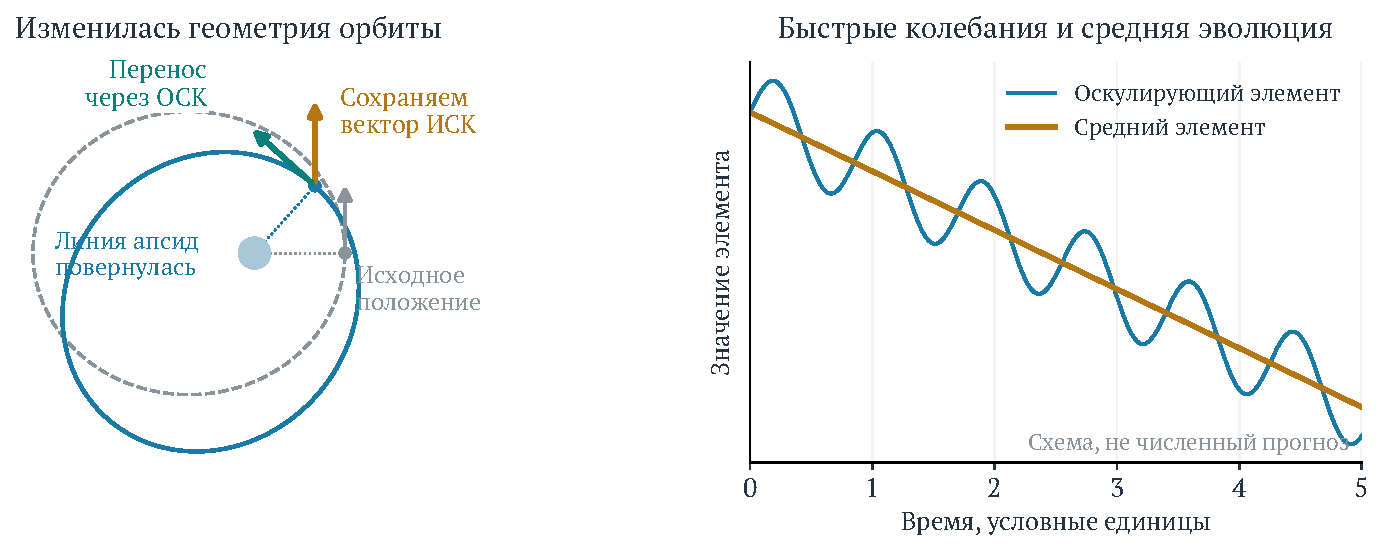
\includegraphics[width=.98\textwidth]{images/perturbed-geometry.pdf}
\caption{Влияние возмущений на перенос
манёвра и представление элементов орбиты. Слева линия апсид
повернулась: прежний инерциальный вектор тяги и направление,
перенесённое вместе с ОСК, различаются. Справа оскулирующий
элемент колеблется около медленно изменяющегося среднего.
Обе части рисунка схематические и не являются результатом
численного расчёта конкретного перехода.}
\label{fig:perturbed-geometry}
\end{figure}

Для размещения манёвра вблизи определённого положения КА
нужен прогноз текущего состояния; одних средних элементов
для этого недостаточно. Если задана средняя целевая орбита,
то и полученную орбиту следует переводить в средние элементы
по той же модели. Сравнение средней цели непосредственно
с оскулирующими элементами может принять периодические
колебания за ошибку перехода.

При оценке оскулирующих элементов результат относят
к одной заданной эпохе $t_f$. Иначе изменение момента оценки
добавляет к изменению от манёвров ещё и изменение самой орбиты
за прошедшее время. В расчётном примере далее сравниваются
оскулирующие элементы в общей конечной эпохе.

\FloatBarrier
\section{Пристрелка с ньютоновским уточнением параметров манёвров}
\label{sec:targeting}

После задания весов, положений и направлений получена
первая последовательность манёвров. Её прогноз с конечной тягой
и возмущениями обычно даёт орбиту, отличающуюся от заданной.
Для устранения этого отличия параметры манёвров уточняют:
сначала оценивают, как они влияют на конечный результат,
затем вычисляют поправку и повторяют прогноз.

\subsection{Невязка и свободные параметры}

Соберём изменяемые параметры в столбец $\vect q$.
Это могут быть длительности манёвров, компоненты их направлений,
положения центров или характеристические скорости групп.
Остальные данные, включая исходное состояние и конечную эпоху,
при уточнении сохраняются.
Для каждого $\vect q$ последовательно рассчитывается вся траектория
и определяется набор конечных величин $\vect y(t_f;\vect q)$.
Невязка равна
\begin{equation}
\vect F(\vect q)=\vect y(t_f;\vect q)-\vect y_{\text{цель}},
\qquad \vect F(\vect q)=0.
\label{eq:residual}
\end{equation}
Состав $\vect y$ задаётся требованиями перехода:
это именно те параметры конечной орбиты или состояния,
которые требуется сформировать.
Для общей оценки величины невязки её компоненты приводят
к согласованной безразмерной форме; конкретная нормировка
задаётся вместе с расчётной задачей.

\subsection{Линеаризация и численное определение производных}

Пусть при текущем выборе $\vect q$ уже известна $\vect F(\vect q)$.
Для малой поправки $\delta\vect q$ разложение первого порядка даёт
\begin{equation}
\vect F(\vect q+\delta\vect q)
\simeq\vect F(\vect q)
 +\frac{\partial\vect F}{\partial\vect q}\,\delta\vect q.
\label{eq:linearize}
\end{equation}
Каждый столбец матрицы $\partial\vect F/\partial\vect q$
показывает изменение всех конечных невязок при изменении
одного параметра манёвров.

Например, выберем $q_1=\tau_1$ --- длительность первого манёвра.
Выполним два полных прогноза, заменив её на $\tau_1+h_1$
и $\tau_1-h_1$ при тех же остальных свободных параметрах.
Тогда первый столбец приближённо равен
\begin{equation}
\frac{\partial\vect F}{\partial\tau_1}
\simeq
\frac{\vect F(\tau_1+h_1,q_2,\ldots)
      -\vect F(\tau_1-h_1,q_2,\ldots)}{2h_1}.
\label{eq:central-difference}
\end{equation}
Изменение первого манёвра влияет на исходные условия всех
последующих участков, поэтому в обоих случаях повторяют
весь расчёт до $t_f$.
Аналогично находят остальные столбцы, меняя по одному параметру.
Шаг $h_k$ должен давать различимое изменение результата,
но оставаться достаточно малым для оценки местной производной.

\subsection{Поправка и повторный прогноз}

Чтобы линейное приближение \eqref{eq:linearize} дало нулевую
невязку, поправку определяют из системы
\begin{equation}
\frac{\partial\vect F}{\partial\vect q}\,\delta\vect q
=-\vect F(\vect q).
\label{eq:newton-correction}
\end{equation}
При равном числе независимых параметров и условий
и невырожденной матрице производных эта система однозначно
задаёт поправку. Если свободных параметров больше, требуется
дополнительное правило выбора: например, поправка наименьшей нормы
в заранее выбранных единицах параметров.

После решения параметры обновляются:
\begin{equation}
\vect q_{\text{нов}}=\vect q+\alpha\,\delta\vect q,
\qquad 0<\alpha\leqslant1.
\label{eq:update}
\end{equation}
Сначала можно проверить полный шаг $\alpha=1$.
Если новый прогноз увеличивает невязку, шаг уменьшают.
После принятого изменения снова рассчитывают траекторию,
вычисляют фактическую невязку и при необходимости заново
определяют производные и поправку. Повторение требуется потому,
что \eqref{eq:linearize} учитывает только первый порядок,
а движение с конечной тягой нелинейно.

Эта последовательность --- метод пристрелки с ньютоновским
уточнением параметров манёвров. Процесс заканчивается при
\begin{equation}
\norm{\vect F(\vect q)}\leqslant\varepsilon,
\label{eq:targeting-stop}
\end{equation}
где $\varepsilon$ --- заданный допуск для выбранного
безразмерного вектора невязки. Малость невязки означает
выполнение конечных требований; минимизация характеристической
скорости потребовала бы отдельного критерия выбора решения.
\FloatBarrier
\section{Расчёт перехода между эллиптическими орбитами}
\label{sec:example}

Соединим рассмотренные приёмы в одном расчёте: построим
двухимпульсное приближение, распределим его между семью
протяжёнными манёврами и уточним их параметры с учётом $J_2$.
Весь прогноз выполняется в классических кеплеровых элементах.
Сравнение последовательных моделей покажет, как конечная длительность
и возмущения изменяют достигнутую орбиту.

\subsection{Исходная и целевая орбиты}

\begin{table}[htbp]
\centering
\renewcommand{\arraystretch}{1.14}
\begin{tabular}{@{}lrr@{}}
\toprule
Элемент & Начальная орбита & Целевая орбита\\\midrule
$a$, км & 18\,500 & 42\,164\\
$e$ & $23/37\simeq0.62162162$ & $0.05$\\
$i$ & $7^\circ$ & $3^\circ$\\
$\Omega$ & $30^\circ$ & $30^\circ$\\
$\omega$ & $0^\circ$ & $0^\circ$\\
$\nu$ & $0^\circ$ & Свободная фаза\\
\bottomrule
\end{tabular}
\caption{Элементы орбит. Целевые значения относятся к общей
конечной эпохе $t_f-t_0=10$ суток.}
\label{tab:inputs}
\end{table}

Начальные радиусы перигея и апогея равны 7000 и 30\,000~км.
Для целевой орбиты они составляют
\[
r_{p,f}=a_f(1-e_f)=40\,055.8~\text{км},\qquad
r_{a,f}=a_f(1+e_f)=44\,272.2~\text{км}.
\]
Начальная масса КА равна 2000~кг, сухая --- 1075~кг;
тяга $F=450$~Н, удельный импульс $I_{\mathrm{sp}}=300$~с.
Используем $\mu=398\,600.4418$~км$^3$/с$^2$,
$R_\oplus=6378.1363$~км, $J_2=1.08262668\cdot10^{-3}$.
Элементы отсчитываются от экваториальной плоскости Земли;
её ось симметрии считается фиксированной.
При интегрировании длины выражаются в километрах, время ---
в секундах; управляющее ускорение переводится в км/с$^2$.

Пять заданных конечных элементов определяют невязку
\begin{equation}
\vect F(\vect q)=
\begin{pmatrix}
(a(t_f;\vect q)-a_f)/a_i\\
e(t_f;\vect q)-e_f\\
i(t_f;\vect q)-i_f\\
\Delta\Omega(t_f;\vect q)\\
\Delta\omega(t_f;\vect q)
\end{pmatrix},
\qquad a_i=18\,500~\text{км}.
\label{eq:kepler-residual}
\end{equation}
Здесь $\Delta\Omega=\Omega-\Omega_f$,
$\Delta\omega=\omega-\omega_f$; разности углов приводятся
к интервалу $[-\pi,\pi)$. Все углы в расчёте выражаются
в радианах. Конечная истинная аномалия не входит в невязку.
Во всех расчётных стадиях используется один критерий:
\begin{equation}
\norm{\vect F(\vect q)}_2\leqslant\varepsilon,
\qquad \varepsilon=10^{-8}.
\label{eq:kepler-criterion}
\end{equation}

\subsection{Уравнения Гаусса и возмущение \texorpdfstring{$J_2$}{J2}}

Интегрируемый столбец имеет вид
\[
\vect z=(a,e,i,\Omega,\omega,\nu,m)^\top.
\]
Обозначим
\begin{equation}
p=a(1-e^2),\qquad h=\sqrt{\mu p},\qquad
r=\frac{p}{1+e\cos\nu},\qquad u=\omega+\nu.
\label{eq:kepler-geometry}
\end{equation}
В этом разделе $S_\Sigma,T_\Sigma,W_\Sigma$ --- компоненты
\emph{суммарного} ускорения от тяги и $J_2$ в текущей ОСК.
Уравнения Гаусса записываются как
\begin{equation}
\begin{aligned}
\dot a&=\frac{2a^2}{h}
 \left(e\sin\nu\,S_\Sigma+\frac{p}{r}T_\Sigma\right),\\
\dot e&=\frac1h\left[p\sin\nu\,S_\Sigma+
 \bigl((p+r)\cos\nu+re\bigr)T_\Sigma\right],\\
\dot i&=\frac{r\cos u}{h}W_\Sigma,\\
\dot\Omega&=\frac{r\sin u}{h\sin i}W_\Sigma,\\
\dot\omega&=\frac{-p\cos\nu\,S_\Sigma+(p+r)\sin\nu\,T_\Sigma}{he}
 -\frac{r\sin u\cos i}{h\sin i}W_\Sigma,\\
\dot\nu&=\frac{h}{r^2}
 +\frac{p\cos\nu\,S_\Sigma-(p+r)\sin\nu\,T_\Sigma}{he},\\
\dot m&=-\frac{F}{c},\qquad c=g_0I_{\mathrm{sp}}.
\end{aligned}
\label{eq:kepler-gauss}
\end{equation}
Истинная аномалия интегрируется непрерывно, без приведения
к одному обороту. Слагаемое $h/r^2$ описывает движение
по орбите; остальные слагаемые учитывают изменение самих элементов.

Компоненты управляющего ускорения равны
$(F/m)(d_r,d_t,d_n)$, где $d_r,d_t,d_n$ --- компоненты
единичного направления тяги в текущей ОСК.
При постоянном инерциальном направлении они пересчитываются
по текущим $\Omega,i,u$.
Положим $K=3J_2\mu R_\oplus^2/(2r^4)$. Тогда
\begin{equation}
\begin{aligned}
S_{J_2}&=K\bigl(3\sin^2i\sin^2u-1\bigr),\\
T_{J_2}&=-K\sin^2i\sin2u,\\
W_{J_2}&=-K\sin2i\sin u,
\end{aligned}
\qquad
\begin{aligned}
S_\Sigma&=\frac{F}{m}d_r+S_{J_2},\\
T_\Sigma&=\frac{F}{m}d_t+T_{J_2},\\
W_\Sigma&=\frac{F}{m}d_n+W_{J_2}.
\end{aligned}
\label{eq:kepler-j2}
\end{equation}
На пассивных участках $F=0$, а возмущающие компоненты
сохраняются. Поэтому между манёврами изменяются и положение
КА на орбите, и элементы орбиты. В модели центрального поля
в \eqref{eq:kepler-j2} полагается $J_2=0$.

\subsection{Двухимпульсное начальное приближение}

Сначала поднимем апогей до $r_{a,f}$, затем в этом апогее
повысим перигей до $r_{p,f}$. Начальная и конечная линии апсид
совпадают с линией узлов, поэтому в тех же точках можно
совместить изменение размера орбиты с уменьшением наклонения.
Промежуточная орбита имеет
\[
a_t=\frac{7000+r_{a,f}}2=25\,636.1~\text{км}.
\]
Скорости в апсидах определяются интегралом энергии:
\begin{equation}
V^2=\mu\left(\frac2r-\frac1a\right).
\label{eq:visviva}
\end{equation}
Обозначим перигейные скорости начальной и промежуточной орбит
через $V_{p,i},V_{p,t}$, апогейные скорости промежуточной
и конечной --- через $V_{a,t},V_{a,f}$.
При уменьшении наклонения на $\delta i$ первым импульсом
\begin{equation}
\begin{aligned}
\Delta V_1(\delta i)&=
\sqrt{(V_{p,t}-V_{p,i})^2+
 4V_{p,t}V_{p,i}\sin^2(\delta i/2)},\\
\Delta V_2(\delta i)&=
\sqrt{(V_{a,f}-V_{a,t})^2+
 4V_{a,f}V_{a,t}\sin^2\!\frac{i_i-i_f-\delta i}{2}}.
\end{aligned}
\label{eq:plane-split}
\end{equation}
Минимизация суммы на $0\leqslant\delta i\leqslant4^\circ$ даёт
$\delta i=\KeplerPlaneOne^\circ$ и
\begin{equation}
\Delta V_1=\KeplerDVOne~\text{м/с},\qquad
\Delta V_2=\KeplerDVTwo~\text{м/с},\qquad
\Delta V_\Sigma=\KeplerDVTotal~\text{м/с}.
\label{eq:nominal-dvs}
\end{equation}
Это минимум в выбранной двухимпульсной апсидальной схеме.
Основной поворот плоскости выполняется в апогее, где ниже
орбитальная скорость. Небольшую часть поворота выгодно
совместить с первым повышением апогея.

\subsection{Веса и размещение семи манёвров}

Первый импульс распределим между тремя манёврами с весами
$(1/3,1/3,1/3)$, второй --- между четырьмя:
\begin{equation}
(w_1,w_2,w_3,w_4)=(0.5848,\ 0.2928,\ 0.1027,\ 0.0197).
\label{eq:kepler-weights}
\end{equation}
Каждый вес задаёт долю характеристической скорости группы.
У перигея КА быстро перемещается, поэтому равные веса ограничивают
максимальную величину отдельного манёвра. Убывающая апогейная
группа оставляет небольшой заключительный манёвр,
абсолютная ошибка которого при относительной модели ошибок меньше.

Эти веса получаются в векторной модели последовательной коррекции
ошибок \cite[§11.1.5--11.1.6]{diprinzio}.
Примем исходный требуемый импульс за единицу.
После каждого манёвра оставшийся требуемый вектор пересчитывается
и распределяется пропорционально оставшимся весам.
При ошибке направления $\theta$ и относительной ошибке величины
$\eta$ получаем
\begin{equation}
\begin{aligned}
W_j&=\sum_{k=j}^Nw_k,\qquad s_j=\frac{w_j}{W_j}\rho_{j-1},
\qquad \rho_0=1,\\
\rho_j&=\sqrt{\rho_{j-1}^2+(1+\eta)^2s_j^2
 -2\rho_{j-1}(1+\eta)s_j\cos\theta}.
\end{aligned}
\label{eq:kepler-weight-model}
\end{equation}
Здесь $\rho_j$ --- модуль требуемого остатка после $j$-го манёвра,
$s_j$ --- запланированная величина очередного манёвра.
Минимизация суммы фактически сообщённых величин и идеальной
коррекции после последнего манёвра,
\begin{equation}
C(\vect w)=\sum_{j=1}^N(1+\eta)s_j+\rho_N,
\qquad \sum_{j=1}^Nw_j=1,\quad w_j\geqslant0,
\label{eq:kepler-weight-objective}
\end{equation}
при $N=4$, $\theta=3^\circ$ и $\eta=0$ воспроизводит
\eqref{eq:kepler-weights}. В данном расчёте ошибки исполнения
не задаются: используется этот демонстрационный профиль весов,
а параметры манёвров уточняются для достижения заданной орбиты.

Длительности всех манёвров находятся по \eqref{eq:duration}.
Равные характеристические скорости первой группы дают разные
длительности из-за изменения массы.

\coursefigure{kepler-groups}{Начальные характеристические скорости
и длительности семи манёвров. Первая группа имеет равные веса,
вторая --- убывающие.}

Манёвры первой группы размещаются около перигея, второй --- около
апогея текущей оскулирующей орбиты. После предыдущего манёвра
по текущей полуоси вычисляется период $P=2\pi\sqrt{a^3/\mu}$.
Пассивный прогноз продолжается не менее $1.5P$;
при переходе ко второй группе --- не менее $2P$.
Затем находится следующее достижение истинной аномалии
\begin{equation}
\nu_{c,1}=0\pmod{2\pi},\qquad
\nu_{c,2}=\pi+\delta\nu\pmod{2\pi}.
\label{eq:kepler-event}
\end{equation}
Его время принимается за центр манёвра $t_c$;
начало назначается на $t_b=t_c-\tau/2$.
Сначала $\delta\nu=0$. Общий сдвиг второй группы затем
уточняется вместе с величинами и направлениями тяги.
Во время каждого манёвра инерциальное направление тяги
постоянно; внутри группы используется одно направление.
Времена центров пересчитываются в каждом новом прогнозе.

\subsection{Конечная длительность и возмущения}

Проследим четыре стадии: аналитическое двухимпульсное решение,
семь протяжённых манёвров в центральном поле,
ту же последовательность с $J_2$ и уточнённую последовательность
с $J_2$. Во всех трёх прогнозах протяжённых манёвров интегрируются
\eqref{eq:kepler-gauss}, а результат оценивается при $t_f=10$ суток.

\begin{table}[htbp]
\centering
\renewcommand{\arraystretch}{1.15}
% Model comparison; terminal norm is dimensionless.
\begin{tabular}{@{}lrrr@{}}
\toprule
Модель & $\|\mathbf F\|_2$ & $\Delta V_\Sigma$, м/с & $m_f$, кг \\
\midrule
Два импульса & $0$ & 1671{,}943 & 1132{,}973 \\
Протяжённые, центр. поле & $1{,}519\cdot10^{-2}$ & 1671{,}943 & 1132{,}973 \\
Протяжённые, $J_2$ & $2{,}465\cdot10^{-1}$ & 1671{,}943 & 1132{,}973 \\
Уточнённые, $J_2$ & $5{,}927\cdot10^{-11}$ & 1712{,}320 & 1117{,}530 \\
\bottomrule
\end{tabular}

\caption{Норма одной и той же невязки и расход на последовательных
стадиях расчёта. В последней строке приведён результат повторного
прогноза с более строгими допусками интегрирования.}
\label{tab:models}
\end{table}

При замене импульсов протяжёнными манёврами суммарная
характеристическая скорость остаётся прежней, но конечная орбита
уже отличается от цели. В центральном поле получаются
$a=\KeplerCentralA$~км, $e=\KeplerCentralE$,
$i=\KeplerCentralI^\circ$; норма невязки равна
$\KeplerNormFiniteCentral$.
При учёте $J_2$ норма возрастает до $\KeplerNormFiniteJTwo$.
При этом $\Omega=\KeplerJTwoOmega^\circ$ и
$\omega=\KeplerJTwoomega^\circ$ вместо заданных $30^\circ$ и $0^\circ$.
Особенно заметно меняются углы, задающие ориентацию орбиты:
линия узлов и линия апсид поворачиваются в течение всего перехода.
Поэтому повторение исходных величин и направлений тяги
на следующих витках требует последующего уточнения.

\coursefigure{kepler-elements}{Эволюция пяти кеплеровых элементов,
задающих конечную орбиту. Сопоставлены исходная последовательность
в центральном поле, та же последовательность с $J_2$ и результат
пристрелки. Истинная аномалия определяет движение КА вдоль орбиты
и в конечных условиях не фиксируется.}

\subsection{Пристрелка и полученная орбита}

Свободными параметрами служат по три компоненты суммарного
приращения скорости каждой группы и сдвиг $\delta\nu$.
Число манёвров и веса сохраняются. После изменения параметров
заново вычисляются длительности, направления тяги и моменты
начала манёвров; затем интегрируется вся последовательность.

Применяем метод пристрелки с ньютоновским уточнением
из главы~\ref{sec:targeting}. Матрица
$\partial\vect F/\partial\vect q$ находится центральными разностями:
для каждого параметра выполняются два полных прогноза.
При пяти условиях и семи параметрах выбираем поправку наименьшей нормы;
при её выборе единицами изменений компонент скорости служат
10~м/с, угла --- 0.05~рад. Если поправка увеличивает невязку
или нарушает ограничения, её уменьшают и повторяют прогноз.

За \KeplerIterations{} ньютоновских шага норма уменьшается
с $\KeplerNormFiniteJTwo$ до $\KeplerNormFinal$.
Минимизация расхода топлива на этом этапе не выполняется.

\coursefigure{kepler-convergence}{Сходимость пристрелки в кеплеровых
элементах по критерию \eqref{eq:kepler-criterion}.
Номер 0 соответствует исходной последовательности с $J_2$.}

Характеристические скорости групп после уточнения равны
$\KeplerTargetGroupOne$ и $\KeplerTargetGroupTwo$~м/с,
сдвиг второй группы --- $\KeplerSiteShift^\circ$.
Направления тяги приведём компонентами в опорных ОСК
двухимпульсного решения: первая ОСК построена в начальном
перигее, вторая --- в апогее промежуточной орбиты.
Компоненты даны в порядке «радиальная, трансверсальная, нормальная»:
\begin{equation}
\vect d_1=\KeplerDirectionOne,\qquad
\vect d_2=\KeplerDirectionTwo.
\label{eq:final-directions}
\end{equation}
Эти опорные базисы фиксируют инерциальные направления групп.
При интегрировании их компоненты пересчитываются в текущую ОСК.

\begin{table}[htbp]
\centering
\small\setlength{\tabcolsep}{5pt}
\renewcommand{\arraystretch}{1.15}
% Seven final finite-thrust manoeuvres.
\begin{tabular}{@{}rrrrr@{}}
\toprule
№ & $t_{b,j}$, сут & $\tau_j$, мин & $\Delta V_j$, м/с & $m_{e,j}$, кг \\
\midrule
1 & 0{,}574791 & 8{,}1368 & 111{,}950 & 1925{,}325 \\
2 & 1{,}243129 & 7{,}8330 & 111{,}950 & 1853{,}438 \\
3 & 2{,}030448 & 7{,}5406 & 111{,}950 & 1784{,}235 \\
4 & 3{,}186469 & 46{,}5374 & 804{,}959 & 1357{,}140 \\
5 & 4{,}521616 & 18{,}9317 & 403{,}030 & 1183{,}395 \\
6 & 6{,}254308 & 6{,}0494 & 141{,}363 & 1127{,}877 \\
7 & 8{,}200499 & 1{,}1275 & 27{,}116 & 1117{,}530 \\
\bottomrule
\end{tabular}

\caption{Параметры найденных протяжённых манёвров.
Времена начала отсчитываются от $t_0$;
направления определены формулой \eqref{eq:final-directions}.}
\label{tab:burns}
\end{table}

Суммарная характеристическая скорость составляет
$\KeplerTargetDVTotal$~м/с, на $\KeplerDVIncrease$~м/с
больше двухимпульсного приближения.
Конечная масса равна $\KeplerFinalMass$~кг:
расходуется $\KeplerFuel$~кг топлива,
остаётся $\KeplerDryReserve$~кг над сухой массой.
Выполнены ограничения на длительности 60--3600~с,
паузы не менее 12~ч и завершение манёвров до $t_f$.

\coursefigure{kepler-timeline}{Тяга и масса в найденной последовательности.
Масса интегрируется в течение каждого протяжённого манёвра.
Между манёврами продолжается возмущённое движение в кеплеровых элементах.}

Повторный прогноз с теми же параметрами и более строгими допусками
интегрирования даёт $\norm{\vect F}_2=\KeplerNormTight<\varepsilon$.
Полученные конечные элементы приведены в таблице~\ref{tab:kepler-final}.

\begin{table}[htbp]
\centering
\renewcommand{\arraystretch}{1.15}
% Target and attained classical elements; tighter Gauss forecast.
\begin{tabular}{@{}lrr@{}}
\toprule
Элемент & Цель & Повторный прогноз \\
\midrule
$a$, км & 42164{,}000000 & 42164{,}000001 \\
$e$ & 0{,}05000000000 & 0{,}05000000000 \\
$i$, град & 3{,}000000000 & 3{,}000000000 \\
$\Omega$, град & 30{,}000000000 & 29{,}999999999 \\
$\omega$, град & 0{,}000000000 & $-1{,}2896\cdot10^{-9}$ \\
$\nu$, град & Свободна & 111{,}967589 \\
\bottomrule
\end{tabular}

\caption{Целевая и полученная орбиты в момент $t_f$.
Результат получен повторным интегрированием уравнений Гаусса
с более строгими допусками.}
\label{tab:kepler-final}
\end{table}

\FloatBarrier
\begin{explanation}{Результат расчёта}
По двухимпульсному решению построена последовательность семи
протяжённых манёвров. Прогноз в кеплеровых элементах показал
отклонение конечной орбиты из-за конечной длительности и $J_2$.
Пристрелка уточнила величины, направления и положения манёвров
и обеспечила заданные $a_f,e_f,i_f,\Omega_f,\omega_f$
в общей конечной эпохе.
\end{explanation}
\FloatBarrier
Расчётные скрипты, исходные параметры, траектории и численные
данные рисунков сохранены в папке \texttt{8/images/}.

\begin{thebibliography}{9}
\addcontentsline{toc}{section}{Литература}
\bibitem{diprinzio}
DiPrinzio M. \textit{Methods of Orbital Maneuvering}.
American Institute of Aeronautics and Astronautics, 2019.
Гл.~11--12: протяжённые манёвры, структура групп, возмущения и пристрелка.
\bibitem{baranov}
Baranov A. \textit{Spacecraft Manoeuvring in the Vicinity of a Near-Circular Orbit}.
Cambridge Scholars Publishing, 2022.
§6.1.1 и 6.1.3: манёвры с постоянным направлением тяги в ОСК и ИСК.
\bibitem{baranov-diss}
Баранов А.~А. \textit{Разработка методов расчета параметров
маневров космических аппаратов в окрестности круговой орбиты}.
Диссертация доктора физико-математических наук. Москва, 2018.
§1.5, 8.4: уточнение решения и маневрирование с конечной тягой.
\bibitem{lecture7}
Чиняев В.~Н. \textit{Задача встречи и относительное движение}.
Методические материалы к лекции 7 курса
«Введение в маневрирование КА», 2026.
\end{thebibliography}
\end{document}
